\documentclass[12pt, letterpaper, twoside]{article}
\usepackage[utf8]{inputenc}
\usepackage[a4paper]{geometry}
\usepackage{array}
\usepackage{booktabs} % For prettier tables
\usepackage{multirow}
\usepackage{multicol}
\usepackage{ragged2e}
\usepackage{xcolor}
\usepackage{gensymb}
\usepackage{fullpage}
\usepackage{hyperref}
\usepackage{amsmath}
\usepackage{scrextend}
\usepackage{graphicx}
\usepackage{lmodern,textcomp}
\usepackage{rotating}
\usepackage[export]{adjustbox}
\usepackage{wrapfig}
\usepackage{subcaption}
\usepackage{caption}

\graphicspath{ {../} }
\newcommand{\cfootnote}[1]{\footnote{\centering #1}}
\title{Venedig: Weltkulturerbe}
\author{Simon Freiermuth \\ \href{mailto:simon@freiermuth.org}{simon@freiermuth.org}}
\date{\today}

\begin{document}

%\begin{titlepage}
\maketitle
%\end{titlepage}

\begin{flushleft}


\section{}
Auf der Fahrt mit unseren Fahrrädern über den Damm von Mestre nach Venedig war
lange gar nichts von Weltkulturerbe zu spüren. Dichter Verkehr, Gestank und Dunst
verdarben uns die Vorfreude fast.


\begin{figure}[h]

\begin{subfigure}{0.5\textwidth}
\hspace{0,5cm}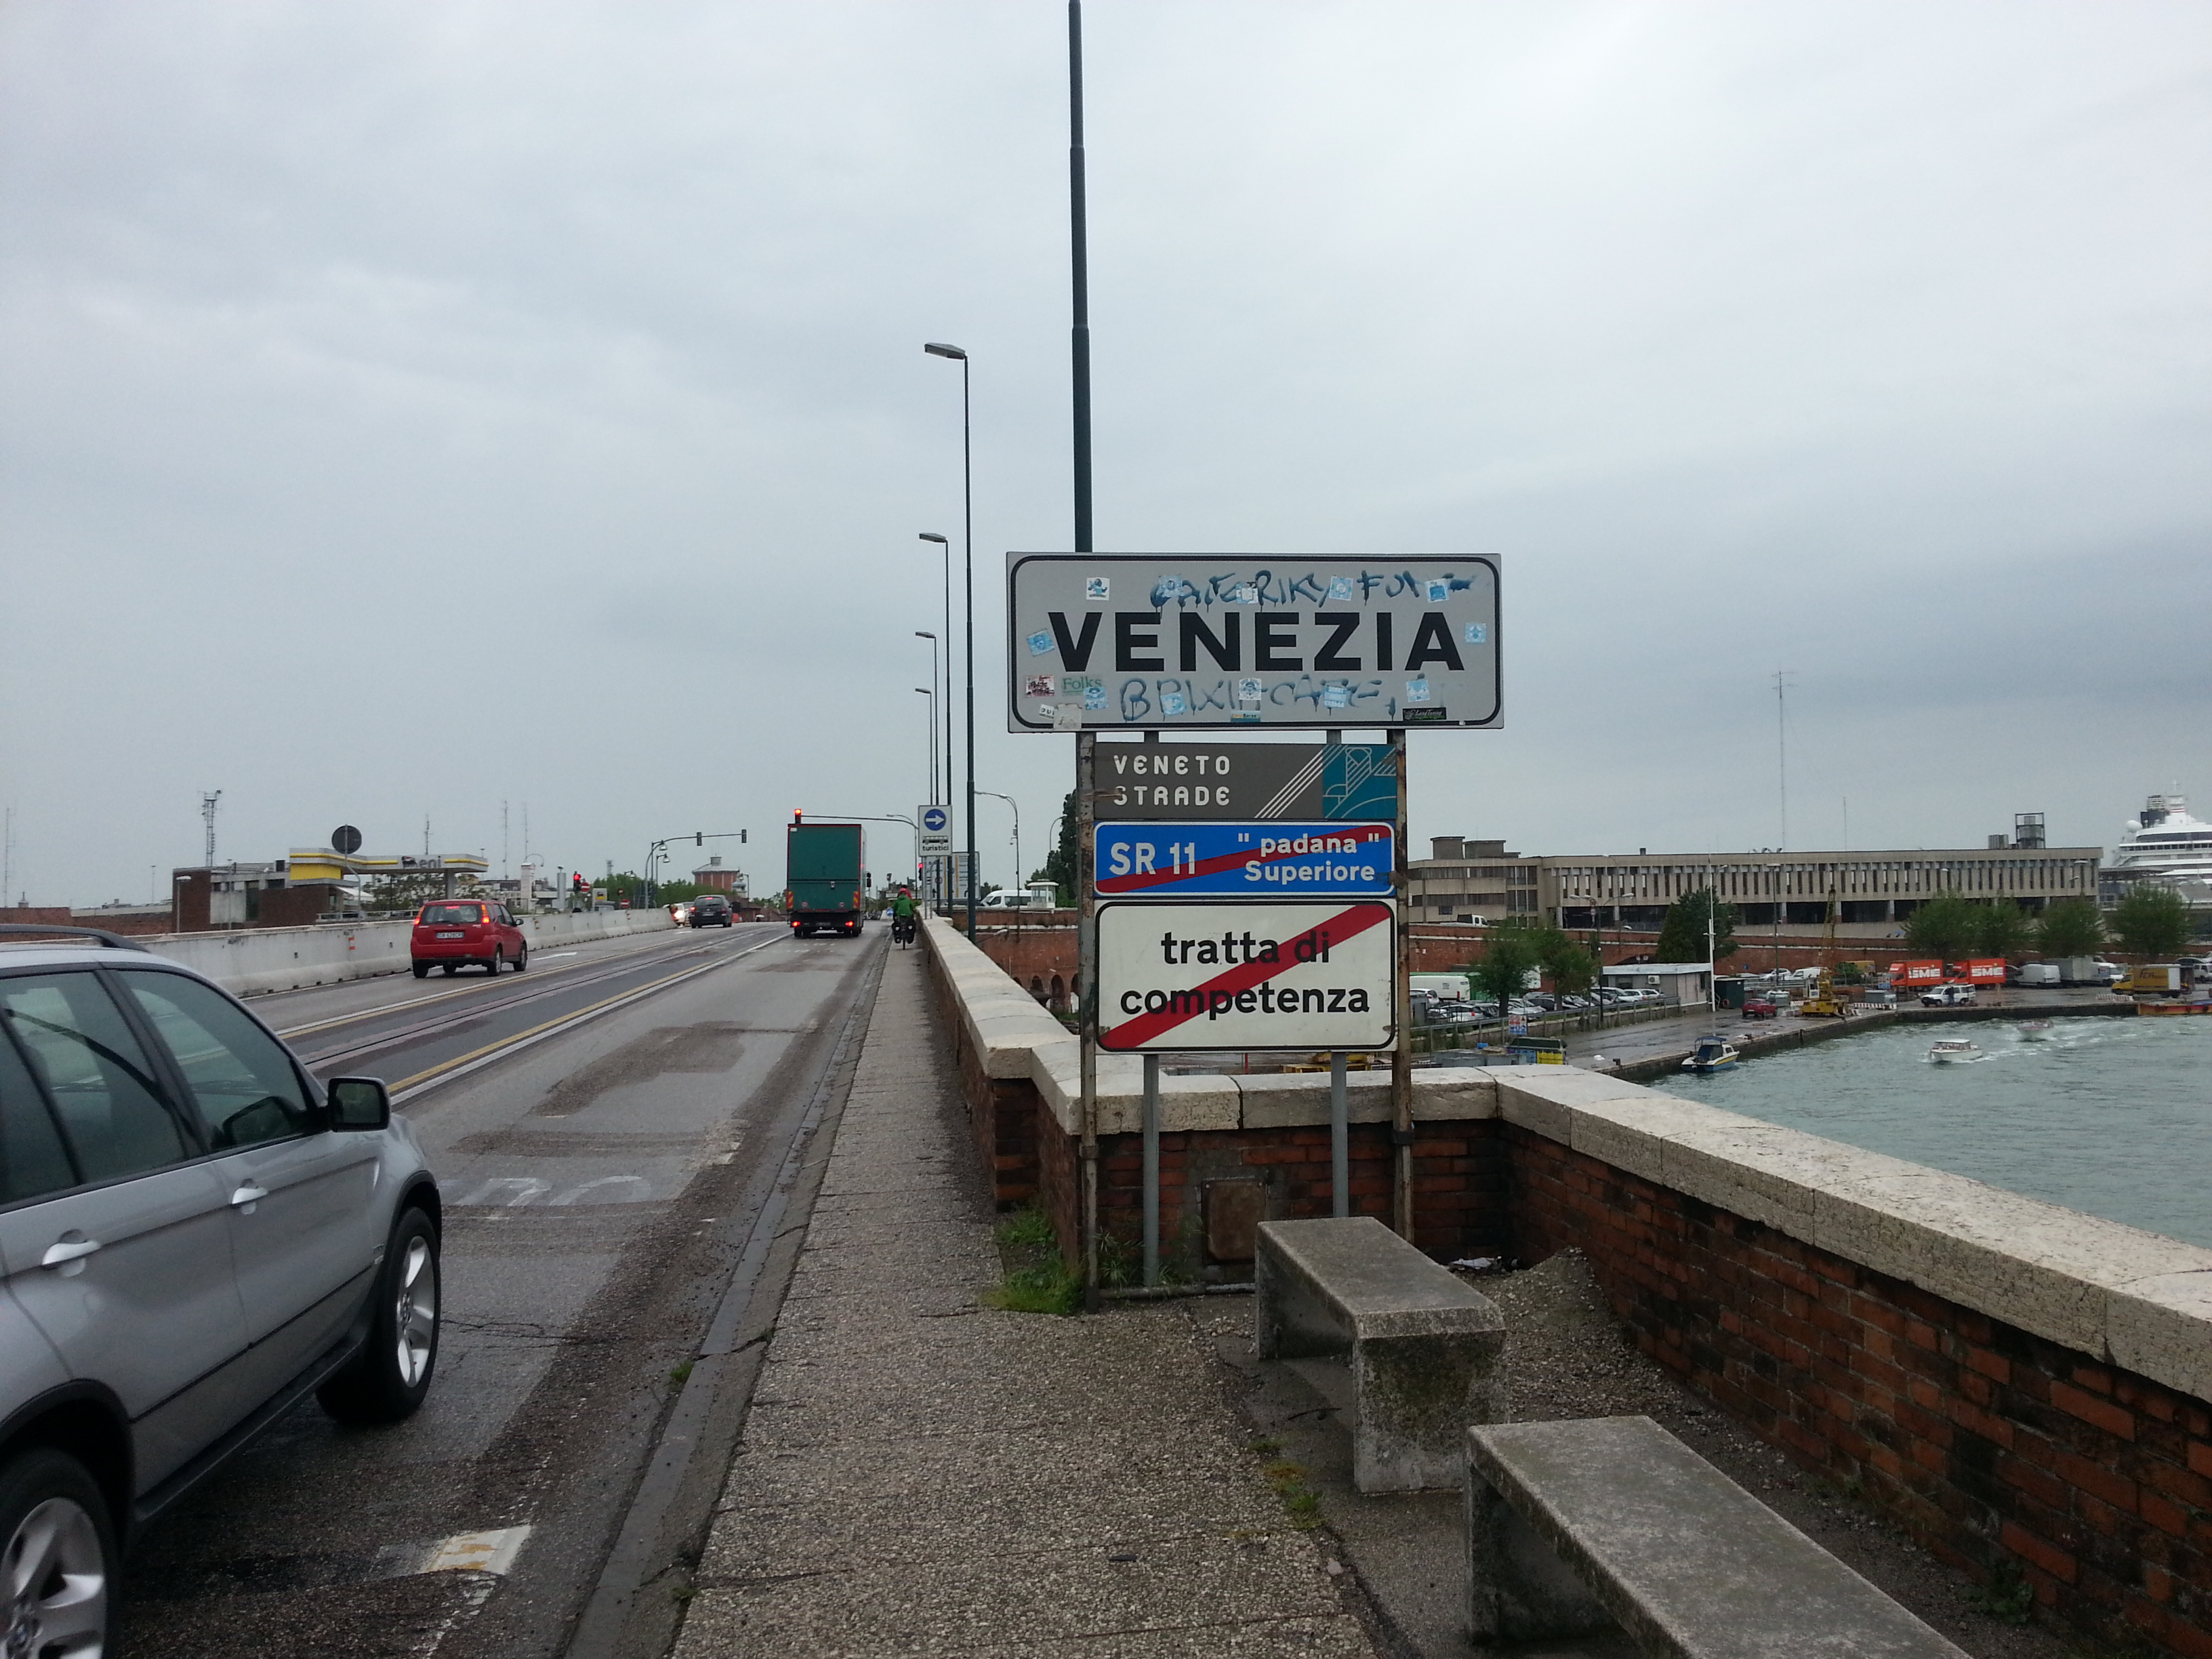
\includegraphics[width=0.9\linewidth, height=5cm]{bild2}
\caption{Und wo ist jetzt die Kultur?}
\end{subfigure}
\begin{subfigure}{0.5\textwidth}
\hspace{1,5cm}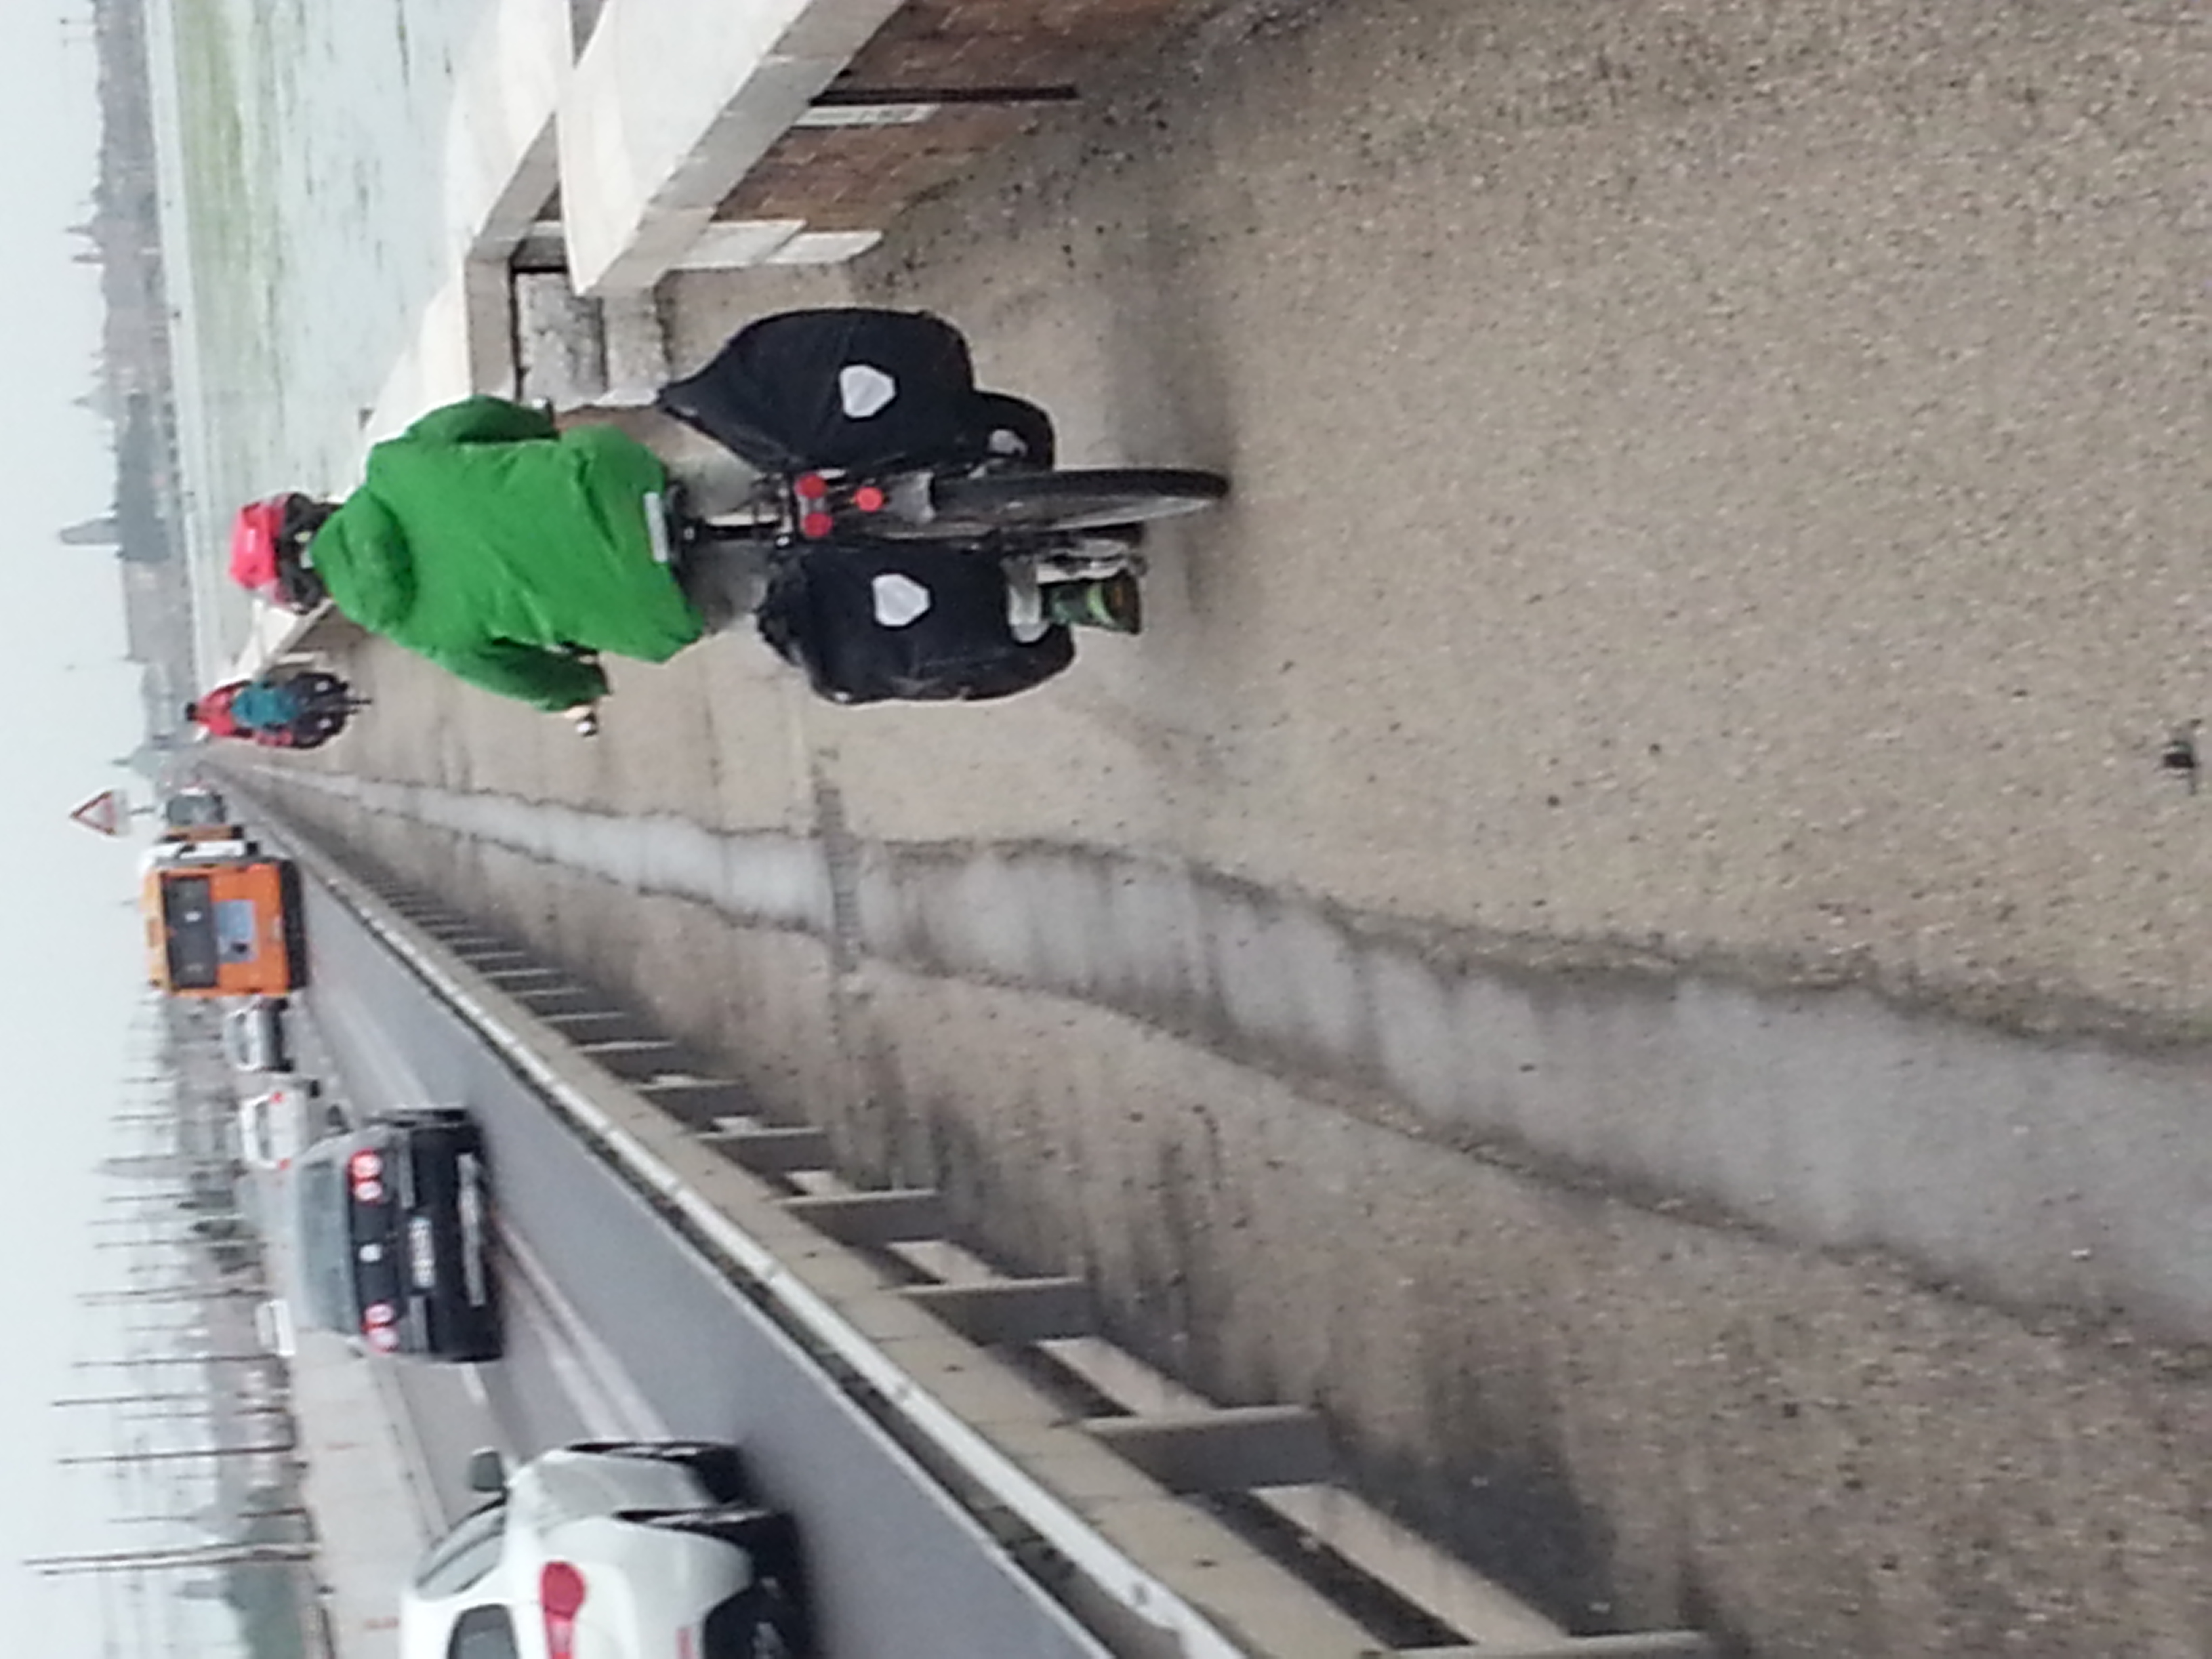
\includegraphics[width=0.9\linewidth, height=5cm, angle=-90]{bild1}
\caption{Das bin ja ich!}
\end{subfigure}

\end{figure}

\pagebreak

Erst als wir mit der Fähre durch den Canale della Giudecca fuhren und einen ersten Blick
auf den Palazzo Ducale warfen, konnten wir erahnen das es hier etwas sehenswertes geben
könnte.

\begin{figure}[h]

\begin{subfigure}{0.5\textwidth}
\hspace{1,5cm}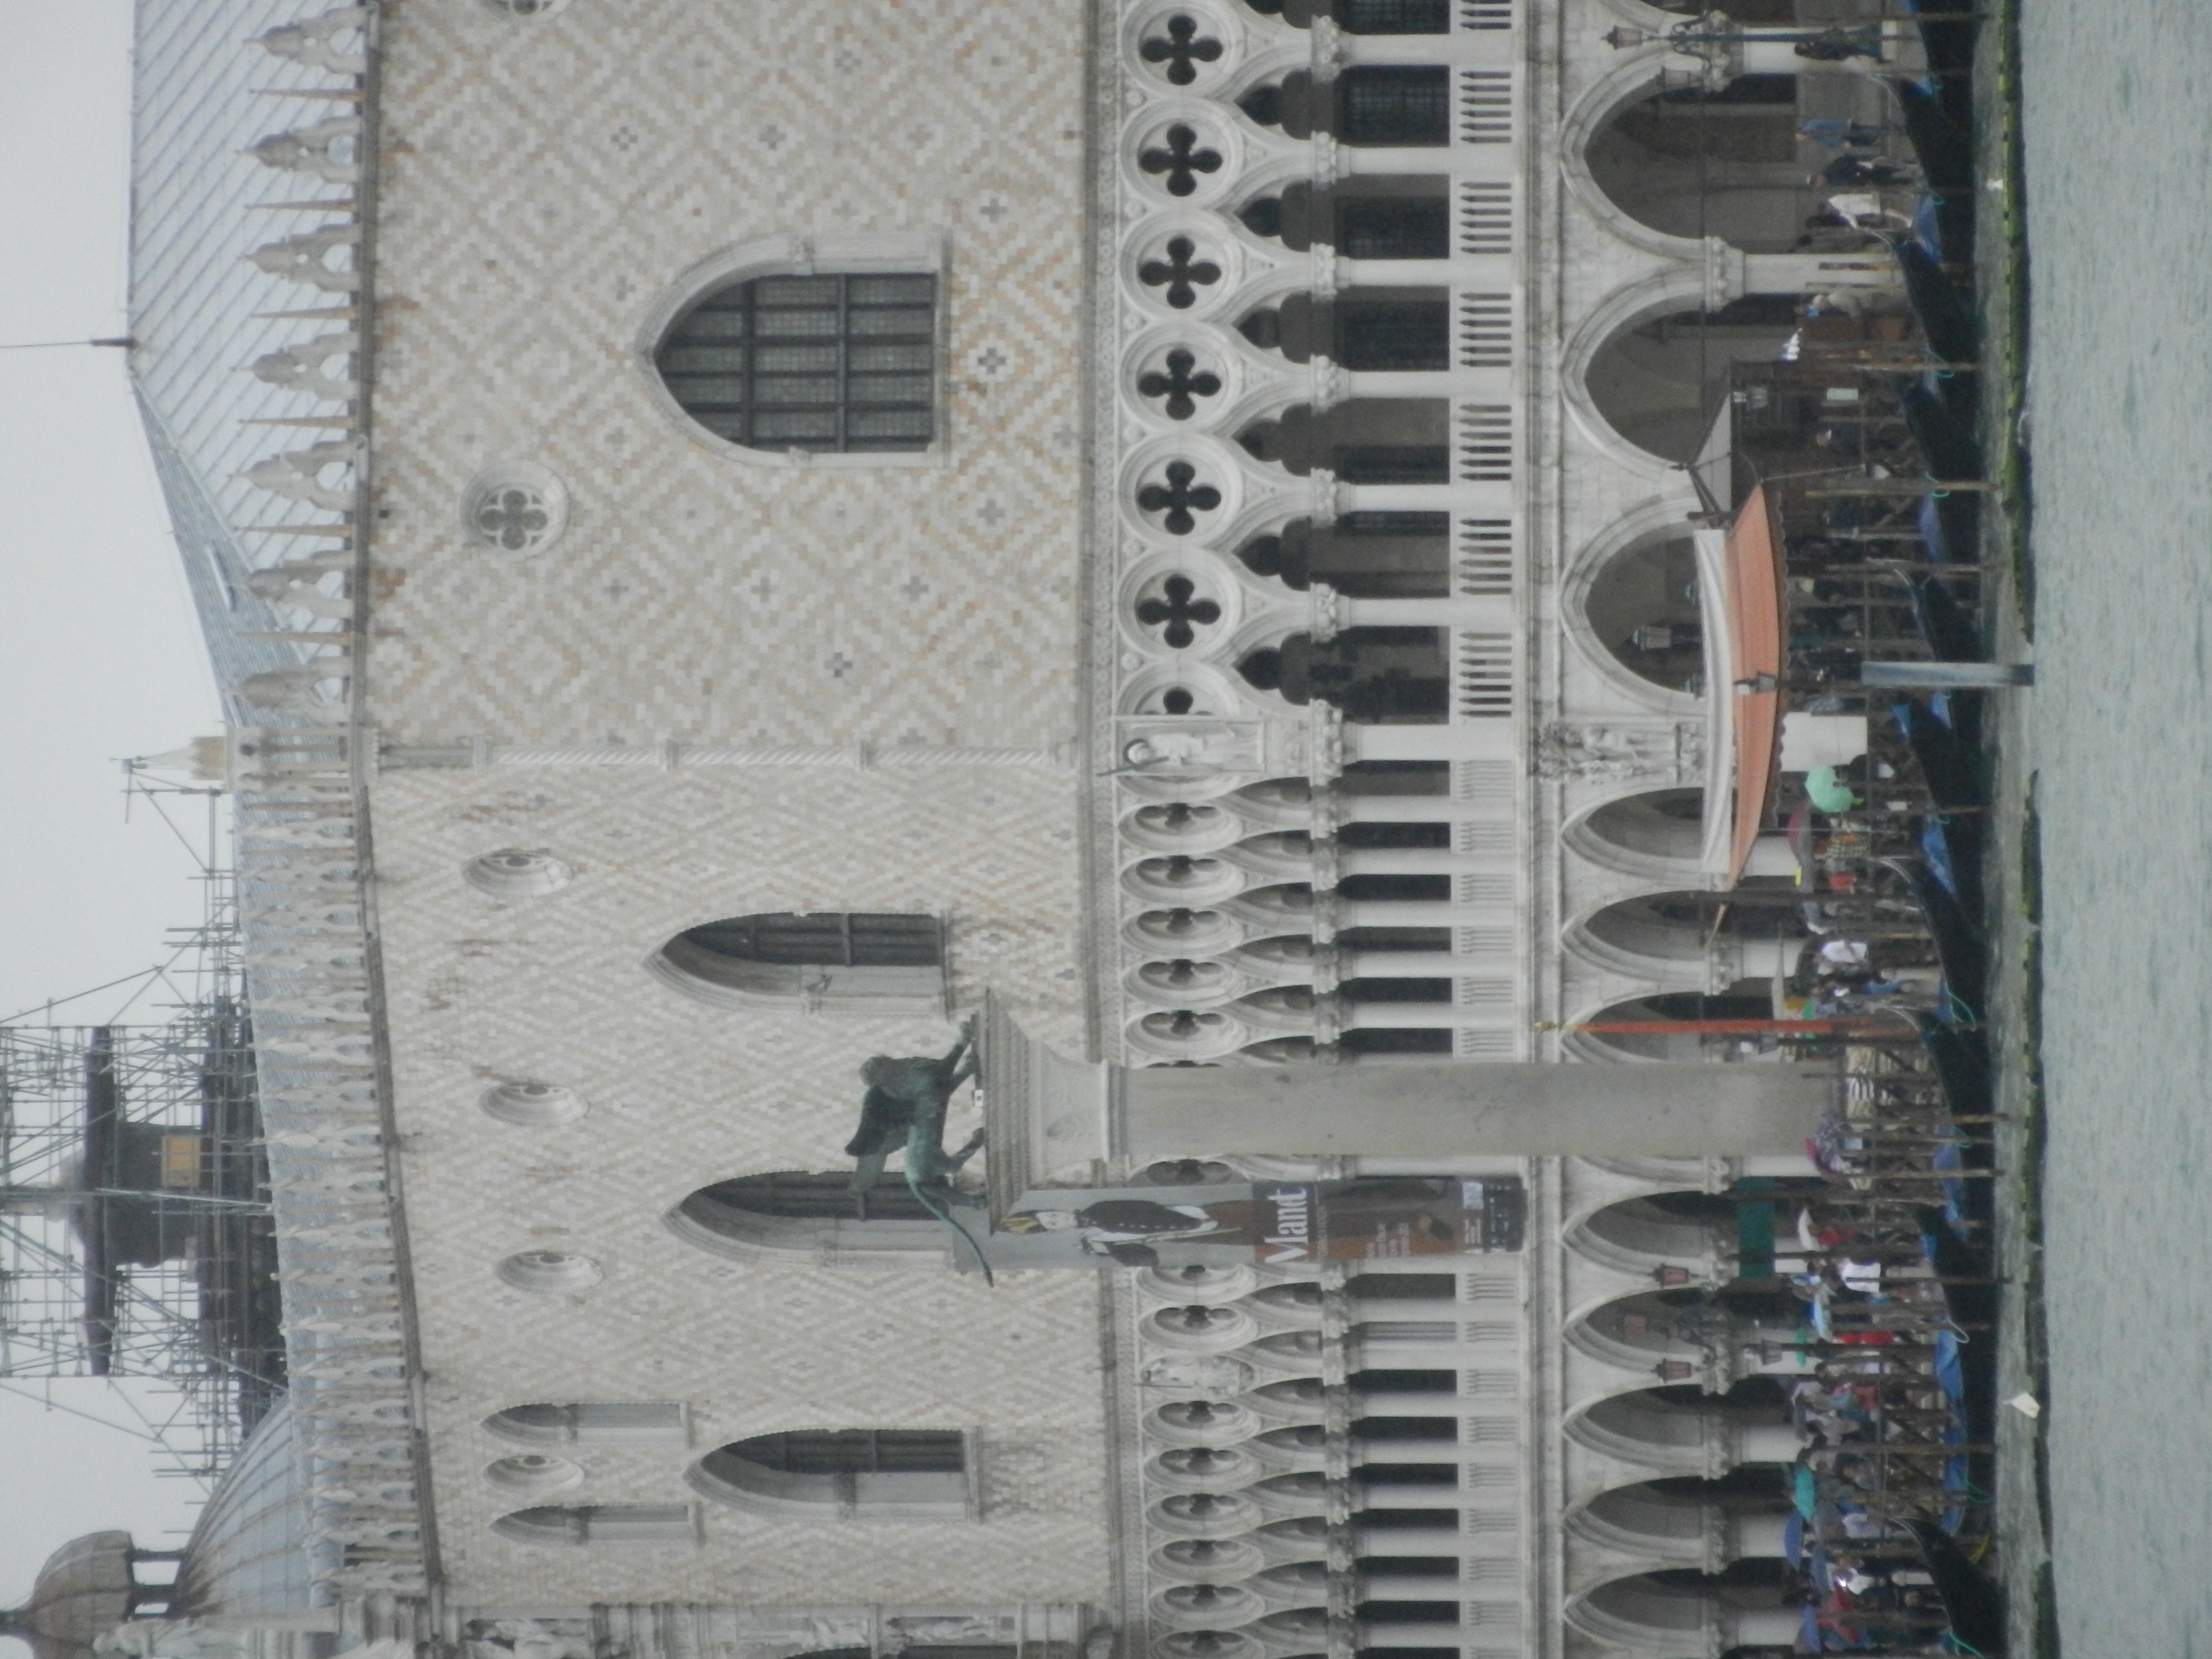
\includegraphics[width=0.9\linewidth, height=5cm, angle=-90]{bild3}
\caption{Palazzo Ducale von der Fähre aus}
\end{subfigure}
\end{figure}

\hfill

Beim Erkunden der Stadt zu Fuss/Gondole haben wir die enorm reichhaltigen Kulturschätze
gesehen

Der Canale Grande ist beeindruckend - die Palazzi der Reichen mit den verschiedenen
Architektonischen Stilen waren eine Augenweide.

Gründung: 500 n.Chr.

Der Verkehr findet grösstenteils auf dem Wasser statt, dies trägt zur speziellen
atmosphäre bei und lässt einen erahnen wie das Leben im Mittelalter war.

Für mich gehört diese Authentizität zum Weltkulturerbe dazu.


\section{}
Wenn viele schwere Amerikaner von den Kreuzfahrtschiffen gleichzeitig in der Stadt sind kann sie sinken,
das Geld von den Hafengebühren geht nach Rom. Und der Konsum der Passagiere in Venedig ist beschränkt,
dies trifft auch auf alle Tagesbesucher zu.


Die öffentliche Infrastruktur ist sehr teuer und wird von den Touristen zusätzlich belastet. Darüber
hinaus werden enorme Mittel (~7Mrd euro) für das Prestigeprojekt MOSE eingesetzt, dessen Nutzen umstritten ist.

Das MOSE Projekt beinhaltet den Bau von einer Trennung des Meeres die Venedig vom Hochwasser schützen soll

Die Wirtschaftliche abhängigkeit vom Tourismus ist sehr hoch, entsprechend ist die durchsetzung von
Einschränkungen wie bspw. Verboten schwierig, zum Beispiel als 2014 das Verbot gegen die allergrössten
Schiffe eingeführt wurde aber bereits 2015 als "rechtswidrig" angesehen wurde. Da kann man sich wundern
wie viel der Richter bekommen hat.


\end{flushleft}

\end{document}
